\documentclass{exam}
\usepackage{graphicx}
\usepackage[utf8]{inputenc}
\usepackage[main=english, vietnamese]{babel}
\usepackage{amsmath}
\usepackage{hyperref}
\usepackage{amsthm}
\usepackage{tcolorbox}
\usepackage{amsfonts}
\usepackage{amssymb}
\usepackage{mathrsfs}
\usepackage{centernot}
\usepackage{multicol}
\usepackage{cases}
\usepackage{physics}
\usepackage[shortlabels]{enumitem}
\usepackage{tasks}
\usepackage{listings}
\usepackage{booktabs}
\usepackage{tikz}
\usetikzlibrary{trees}

\setlength{\heavyrulewidth}{1.5pt}
\setlength{\abovetopsep}{4pt}

\tikzstyle{level 1}=[level distance=5cm, sibling distance=4cm]
\tikzstyle{level 2}=[level distance=5cm, sibling distance=4cm]
\tikzstyle{level 2}=[level distance=5cm, sibling distance=4cm]
\tikzstyle{end} = [circle, minimum width=5pt,fill, inner sep=0pt]

\definecolor{borderblue}{HTML}{33c2ff}
\definecolor{codegreen}{rgb}{0,0.6,0}
\definecolor{codegray}{rgb}{0.5,0.5,0.5}
\definecolor{codepurple}{rgb}{0.58,0,0.82}
\definecolor{backcolour}{rgb}{0.95,0.95,0.92}

\lstdefinestyle{mystyle}{
    backgroundcolor=\color{backcolour},   
    commentstyle=\color{codegreen},
    keywordstyle=\color{magenta},
    numberstyle=\tiny\color{codegray},
    stringstyle=\color{codepurple},
    basicstyle=\ttfamily\footnotesize,
    breakatwhitespace=false,         
    breaklines=true,                 
    captionpos=b,                    
    keepspaces=true,                 
    numbers=left,                    
    numbersep=5pt,                  
    showspaces=false,                
    showstringspaces=false,
    showtabs=false,
    tabsize=2
}

\lstset{style=mystyle}

\newcommand{\paren}[1]{\left(#1\right)}
\newcommand{\curly}[1]{\left\{#1\right\}}
\newcommand{\lxor}{\oplus}
\newcommand{\Mid}{\;\middle|\;}

\allowdisplaybreaks

\makeatletter
\renewcommand*\env@matrix[1][*\c@MaxMatrixCols c]{%
  \hskip -\arraycolsep
  \let\@ifnextchar\new@ifnextchar
  \array{#1}}
\makeatother

\makeatletter
\long\def\paragraph{%
  \@startsection{paragraph}{4}%
  {\z@}{2ex \@plus 1ex \@minus .2ex}{-1em}%
  {\normalfont\normalsize\bfseries}%
}
\makeatother

\makeatletter
\def\@xequals@fill{\arrowfill@\Relbar\Relbar\Relbar}
\newcommand*\xequals[2][]{\DOTSB\ext@arrow0055\@xequals@fill{#1}{#2}}
\makeatother

\DeclareMathOperator{\lcm}{lcm}
\DeclareMathOperator{\spn}{span}
\DeclareMathOperator{\im}{im}
\DeclareMathOperator{\nullity}{nullity}

\NewTColorBox{problem}{m}{
  standard jigsaw,
  sharp corners,
  boxrule=0.4pt,
  coltitle=black,
  colframe=black,
  opacityback=0,
  opacitybacktitle=0,
  fonttitle=\normalfont\bfseries\upshape,
  fontupper=\normalfont,
  title={Problem #1},
  after title={.},
  attach title to upper={\ },
}

\title{STAT451 - Homework 2}
\author{\foreignlanguage{vietnamese}{Trần Tôn Minh Kỳ}}
\date{\today}

\begin{document}

\maketitle

\begin{problem}{83}
	Consider numerical observations $x_1, \dots, x_n$. It is frequently of interest to know whether the $x_i$'s are (at least approximately) symmetrically distributed about some value. If $n$ is at least moderately large, the extent of symmetry can be assessed from a stem-and-leaf display or histogram. However, if $n$ is not very large, such pictures are not particularly informative. Consider the following alternative. Let $y_1$ denote the smallest $x_i$, $y_2$ the second smallest $x_i$, and so on. Then plot the following pairs as points on a two-dimensional coordinate system: $(y_n - \widetilde{x}, \widetilde{x} - y_1), (y_{n - 1} - \widetilde{x}, \widetilde{x} - y_2), (y_{n - 2} - \widetilde{x}, \widetilde{x} - y_3), \dots$. There are $n/2$ points when $n$ is even and $(n - 1)/2$ when $n$ is odd.
	\begin{tasks}[label=\textbf{\alph*.}]
		\task What does this plot look like when there is perfect symmetry in the data? What does it look like when observations stretch out more above the median than below it (a long upper tail)?
		\task The accompanying data on rainfall (acre-feet) from 26 seeded clouds is taken from the article \textbf{``A Bayesian Analysis of a Multiplicative Treatment Effect in Weather Modification (\textit{Technometrics}, 1975: 161--166)''}. Construct the plot and comment on the extent of symmetry or nature of departure from symmetry.
		\begin{center}
			\begin{tabular}{ccccccc}
				4.1 & 7.7 & 17.5 & 31.4 & 32.7 & 40.6 & 92.4 \\
				115.3 & 118.3 & 119.0 & 129.6 & 198.6 & 200.7 & 242.5 \\
				255.0 & 274.7 & 274.7 & 302.8 & 334.1 & 430.0 & 489.1 \\
				703.4 & 978.0 & 1656.0 & 1697.8 & 2745.6
			\end{tabular}
		\end{center}
	\end{tasks}
\end{problem}

\paragraph{a.} When there is perfect symmetry in the data, all the points lie on the graph of the equation $y = x$. This makes sense since it shows all elements are perfectly distributed about the median. As the observations stretch more above the median, the set of points has a tendency to stretch out horizontally. More formally, the linear regression of $\{(y_{n - i + 1} - \widetilde{x}, \widetilde{x} - y_i)\}$ has a slope below $1$.

\paragraph{b.} The pointset plot of the data is shown as follows. An additional dashed red line is drawn as the graph of the equation $y = x$, and a solid blue line as the linear regression of the dataset.
\begin{center}
	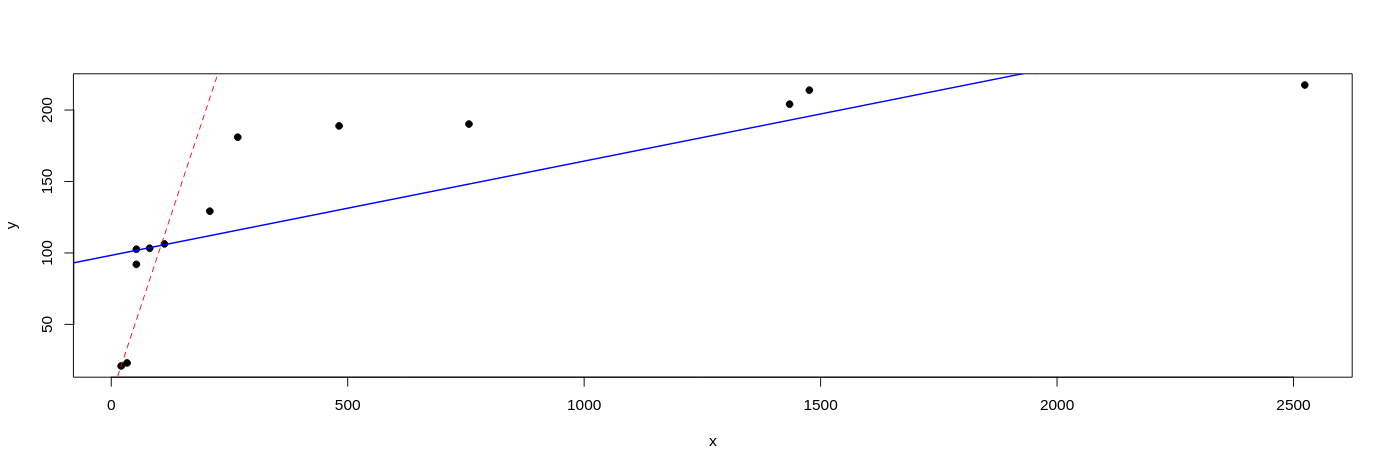
\includegraphics[scale=0.3]{img/83.png}
\end{center}

Based on the plot, one can see that the dataset is asymmetrical. More specifically, data is more spread out above the median, leading to a lower slope of the linear regression. Because of the extent to which the regression skew away from the $y = x$ line, one may interpret that the dataset greatly departs from symmetry.

\begin{problem}{94}
	A transmitter is sending a message by using a binary code, namely, a sequence of $0$'s and $1$'s. Each transmitted bit ($0$ or $1$) must pass through three relays to reach the receiver. At each relay, the probability is $.20$ that the bit sent will be different from the bit received (a reversal). Assume that the relays operate independently of one another.
	\[
		\text{Transmitter} \longrightarrow \text{Relay 1} \longrightarrow \text{Relay 2} \longrightarrow \text{Relay 3} \longrightarrow \text{Receiver}
	\]
	\begin{tasks}[label=\textbf{\alph*.}]
		\task If a $1$ is sent from the transmitter, what is the probability that a $1$ is sent by all three relays?
		\task If a $1$ is sent from the transmitter, what is the probability that a $1$ is received by the receiver?
		\task Suppose $70\%$ of all bits sent from the transmitter are $1$s. If a $1$ is received by the receiver, what is the probability that a $1$ was sent?
	\end{tasks}
\end{problem}

We preface the solution by denoting $R_i$ to be the event of a reversal occuring in relay $i$, thus $P(R_1) = P(R_2) = P(R_3) = .20$.

\paragraph{a.} For a $1$ to be sent by all three relays, there must not be any reversal occured; i.e., the probability that a $1$ is sent by all three relays is $P(\overline{R_1} \cap \overline{R_2} \cap \overline{R_3})$. Because the $R_i$'s are mutually independent, so are the $\overline{R_i}$'s. We thus obtain that
\[
	P(\overline{R_1} \cap \overline{R_2} \cap \overline{R_3}) = P(\overline{R_1})P(\overline{R_2})P(\overline{R_3}) = (1 - .20)^3 = .512.
\]

\paragraph{b.} One can observe that for the receiver to receive a $1$, no reversal or exactly two reversals among three relays must occur. The probability for the former to occur is .512 as shown in \textbf{94a}. We now calculate the probability for the latter event to occur. Let $S_I$ be the events where all relays $i \in I$ have a reversal occur. Observe that for each 2-subset $I \subseteq \{1, 2, 3\}$,
\[
	P(S_I) = P\paren{\bigcap_{i \in I} R_i \cap \bigcap_{j \notin I} \overline{R_j}} = .20^2 \times .80^1 = .032.
\]
The probability for precisely two relays to have a reversal occur is thus
\[
	\binom32 P(S_I) = .096.
\]
By the Kolmogorov's third axiom, the probability that a $1$ is received by the receiver is $.512 + .096 = .608$.

\paragraph{c.} Denote $A$ and $B$ to be the following events:
\[
	A: \text{1 is received by the receiver,} \qquad B: \text{1 is sent from the transmitter}.
\]
Then $P(B) = .70$. From \textbf{94b}, we obtain that $P(A \mid B) = .608$. Thus we need to calculate $P(B \mid A)$. To this end, we first calculate $P(A \mid \overline{B})$, i.e. the probability of the receiver receiving a $1$ if a $0$ is sent from the transmitter. Using the same argument as \textbf{94a} and \textbf{94b}, one can readily show that for 1-subsets $I \subseteq \{1, 2, 3\}$,
\[
	P(A \mid \overline{B}) = P(R_1 \cap R_2 \cap R_3) + \binom31 P\paren{\bigcap_{i \in I} R_i \cap \bigcap_{j \notin I} \overline{R_j}} = .392.
\]
From this, we are able to calculate $P(A)$ using the law of total probability:
\[
	P(A) = P(A \mid B)P(B) + P(A \mid \overline{B})P(\overline{B}) = .608 \times .7 + .392 \times (1 - .7) = .5432.
\]
Finally we use Bayes's theorem to calculate $P(B \mid A)$:
\[
	P(B \mid A) = \frac{P(A \mid B)P(B)}{P(A)} = \frac{.608 \times .70}{.716} \approx .7835.
\]

\begin{problem}{95}
	Individual A has a circle of five close friends (B, C, D, E, and F). A has heard a certain rumor from outside the circle and has invited the five friends to a party to circulate the rumor. To begin, A selects one of the five at random and tells the rumor to the chosen individual. That individual then selects at random one of the four remaining individuals and repeats the rumor. Continuing, a new individual is selected from those not already having heard the rumor by the individual who has just heard it, until everyone has been told.
	\begin{tasks}[label=\textbf{\alph*.}]
		\task What is the probability that the rumor is repeated in the order B, C, D, E, and F?
		\task What is the probability that F is the third person at the party to be told the rumor?
		\task What is the probability that F is the last person to hear the rumor?
		\task If at each stage the person who currently ``has'' the rumor does not know who has already heard it and selects the next recipient at random from all five possible individuals, what is the probability that F has still not heard the rumor after it has been told ten times at the party?
	\end{tasks}
\end{problem}

For \textbf{95a}, \textbf{95b}, \textbf{95c}, define $\mathcal S$ to be the sample space. One may interpret a sequence of any distinct letter from B to F to be the order of people being told the rumor (thus all sequence in $\mathcal S$ has a length of 5). Thus one can readily show that $\abs{\mathcal S} = 5! = 120$.

\paragraph{a.} Since there is precisely one sequence satisfying this condition (BCDEF), the probability that the rumor is repeated in the given order of people is
\[
	\frac{1}{120} \approx .0083.
\]

\paragraph{b.} The number of sequences in the form \_\_F\_\_ is clearly $4! = 24$. Thus the probability that F is the third person to be told the rumor is
\[
	\frac{24}{120} = .2.
\]

\paragraph{c.} The same argument in \textbf{95b} can be used to find the number of sequences in the form \_\_\_\_F and so the probability that F is the last person to be told the rumor is also $.2$.

\paragraph{d.} Because the last person to be told the rumor does not know who has already heard it, the letters no longer need not be unique. We first calculate the number of such sequences with length $10$, which is simply $5^{10}$. The number of sequences with length $10$ excluding F is $4^{10}$, thus the probability F has not heard the rumor after it has been told ten times is
\[
	\frac{4^{10}}{5^{10}} \approx .1074.
\]

\begin{problem}{96}
	According to the article \textbf{``Optimization of Distribution Parameters for Estimating Probability of Crack Detection'' (\textit{J. of Aircraft}, 2009: 2090--2097)}, the following ``Palmberg'' equation is commonly used to determine the probability $P_d(c)$ of detecting a crack of size $c$ in an aircraft structure:
	\[
		P_d(c) = \frac{(c/c^*)^\beta}{1 + (c/c^*)^\beta}
	\]
	where $c^*$ is the crack size that corresponds to a .5 detection probability (and thus is an assessment of the quality of the inspection process).
	\begin{tasks}[label=\textbf{\alph*.}]
		\task Verify that $P_d(c^*) = .5$
		\task What is $P_d(2c^*)$ when $\beta = 4$?
		\task Suppose an inspector inspects two different panels, one with a crack size of $c^*$ and the other with a crack size of $2c^*$. Again assume $\beta = 4$ and also that the results of the two inspections are independent of one another, what is the probability that exactly one of the two cracks will be detected?
		\task What happens to $P_d(c)$ as $\beta \to \infty$?
	\end{tasks}
\end{problem}

\paragraph{a.} We substitute $c^*$ into $P_d(c)$ and obtain that
\[
	P_d(c^*) = \frac{1^\beta}{1 + 1^\beta} = \frac12 = .5.
\]

\paragraph{b.} We substitute $2c^*$ to $P_d(c)$ and assume $\beta = 4$. We thus obtain that
\[
	P_d(2c^*) = \frac{(2c^*/c^*)^4}{1 + (2c^*/c^*)^4} \approx .9412.
\]

\paragraph{c.} By \textbf{96a} and \textbf{96b}, we obtain $P_d(c^*) = .5$ and $P_d(2c^*) \approx .9412$. Thus the probability that exactly one event out of the two events will happen is $.5(1 - .9412) + .9412(1 - .5) = .5$ (this equation makes sense since the two inspections are mutually independent).

\paragraph{d.} Using a change of variable $\beta \mapsto (c/c*)^\beta$, we evaluate the following limit:
\[
	\lim_{\beta \to \infty} \frac{(c/c^*)^\beta}{1 + (c/c^*)^\beta} = \lim_{\beta \to \infty} \frac{\beta}{1 + \beta} = 1.
\]
Thus, as $\beta$ approaches infinity, the probability $P_d(c)$ approaches $1$.

\begin{problem}{97}
	A chemical engineer is interested in determining whether a certain trace impurity is present in a product. An experiment has a probability of .80 of detecting the impurity if it is present. The probability of not detecting the impurity if it is absent is .90. The prior probabilities of the impurity being present and being absent are .40 and .60, respectively. Three separate experiments result in only two detections. What is the posterior probability that the impurity is present?
\end{problem}

Denote by $A$ and $B$ the events
\[
	A: \text{Impurity is present,} \qquad B: \text{The experiment detects impurity (positive)}.
\]

A probability tree diagram is thus given below.
\begin{center}
	\begin{tikzpicture}[grow=right, sloped]
	\node[end] {}
		child {
			node[end] {}        
				child {
					node[end] {}
					edge from parent
					node[above] {Negative}
					node[below]  {$P(\overline{B} \mid \overline{A}) = .9$}
				}
				child {
					node[end] {}
					edge from parent
					node[above] {Positive}
					node[below]  {$P(B \mid \overline{A}) = .1$}
				}
				edge from parent 
				node[above] {Not present}
				node[below]  {$P(\overline{A}) = .6$}
		}
		child {
			node[end] {}        
			child {
					node[end] {}
					edge from parent
					node[above] {Negative}
					node[below]  {$P(\overline{B} \mid A) = .2$}
				}
				child {
					node[end] {}
					edge from parent
					node[above] {Positive}
					node[below]  {$P(B \mid A) = .8$}
				}
			edge from parent         
				node[above] {Present}
				node[below]  {$P(A) = .4$}
		};
	\end{tikzpicture}
\end{center}
Applying the law of total probability, one can see that
\[
	P(B) = P(B \mid A)P(A) + P(B \mid \overline{A})P(\overline{A}) = .8 \times .4 + .1 \times .6 = .38.
\]
We now calculate the probability for exactly two detections to occur out of three experiments. To this end, we define $C$ to be the event of exactly two experiments to return positive and $B_i$ to be the event of experiment $i \in \{1, 2, 3\}$ returning positive. Using this notation, the quantity we need to solve for is $P(A \mid C)$. Now observe that
\[
	P(C \mid A) = \sum_{I\subseteq\{1, 2, 3\}}P\paren{\bigcap_{i \in I} B_i \cap \bigcap_{j \notin I} \overline{B_j} \Mid A} = \binom32(.8^2 \times .2^1) = .384.
\]
Additionally,
\[
	P(C \mid \overline{A}) = \sum_{I\subseteq\{1, 2, 3\}}P\paren{\bigcap_{i \in I} B_i \cap \bigcap_{j \notin I} \overline{B_j} \Mid \overline{A}} = \binom32(.1^2 \times .9^1) = .027.
\]
We now apply Bayes's theorem to calculate $P(A \mid C)$:
\[
	P(A \mid C) = \frac{P(C \mid A)P(A)}{P(C)} = \frac{P(C \mid A)P(A)}{P(C \mid A)P(A) + P(C \mid \overline A)P(\overline A)} \approx .9046
\]

\begin{problem}{98}
	Five friends---Allison, Beth, Carol, Diane, and Evelyn---have identical calculators and are studying for a statistics exam. They set their calculators down in a pile before taking a study break and then pick them up in random order when they return from the break. What is the probability that at least one of the five gets her own calculator?
\end{problem}

Denote by $A$, $B$, $C$, $D$, and $E$ the events where Allison, Beth, Carol, Diane, and Evelyn get her own calculators, respectively. Then the probability of each event is clearly $.2$. We dutifully note that as an event occurs, the sample space dynamically changes. More specifically, regardless of the outcome of any event $A$, $B$, $C$, $D$ and $E$, the sample space reduces by $1$. It is thus useful that we calculate the general probability for events intersections. Let $U = \{A, B, C, D, E\}$; for any $I \subseteq U$, we obtain that:
\[
	P\paren{\bigcap_{X \in I} X} = \prod_{i = 1}^{\abs{X}}\frac{1}{5 - i + 1} = \frac{(5 - \abs{X})!}{5!}.
\]
We now solve for the probability that at least one of the five friends gets her own calculator.
\begin{align*}
	P\paren{\bigcup_{X \in U} X} &= \sum_{i = 1}^5 \paren{(-1)^{i + 1}\binom5i \frac{(5 - i)!}{5!}} = \sum_{i = 1}^5 \frac{(-1)^{i + 1}}{i!} \\
	&= \frac11 - \frac1{1 \cdot 2} + \frac1{1 \cdot 2 \cdot 3} - \frac1{1 \cdot 2 \cdot 3 \cdot 4} + \frac1{1 \cdot 2 \cdot 3 \cdot 4 \cdot 5} \\
	&\approx .6333.
\end{align*}

\paragraph{Remark.} This approach is easily extendible to an arbitrary $n$ individuals. As a matter of fact, as $n \to \infty$, $P(\bigcup U)$ converges by the alternating series test.
\begin{align*}
	\sum_{i = 1}^\infty \frac{(-1)^{i + 1}}{i!} = 1 - \frac1e \approx .6321.
\end{align*}

\begin{problem}{99}
	Fasteners used in aircraft manufacturing are slightly crimped so that they lock enough to avoid loosening during vibration. Suppose that $95\%$ of all fasteners pass an initial inspection. Of the $5\%$ that fail, $20\%$ are so seriously defective that they must be scrapped. The remaining fasteners are sent to a recrimping operation, where $40\%$ cannot be salvaged and are discarded. The other $60\%$ of these fasteners are corrected by the recrimping process and subsequently pass inspection.
	\begin{tasks}[label=\textbf{\alph*.}]
		\task What is the probability that a randomly selected incoming fastener will pass inspection either initially or after recrimping?
		\task Given that a fastener passed inspection, what is the probability that it passed the initial inspection and did not need recrimping?
	\end{tasks}
\end{problem}

\paragraph{a.} Denote $A$, $B$ and $C$ to be the following statements:
\[
	A: \text{Fastener passes initial inspection,} \quad B: \text{Fastener is scrapped,} \quad C: \text{Fastener is discarded.}
\]
We wish to calculate $P(A \cup (\overline{A} \cap \overline{B} \cap \overline{C}))$. To this end, we use the inclusion-exclusion principle.
\[
	P(A \cup (\overline{A} \cap \overline{B} \cap \overline{C})) = P(A) + P(\overline{A} \cap \overline{B} \cap \overline{C}).
\]
The intersection term is omitted because it contains $A \cap \overline{A}$, resulting in an empty set. A probability tree diagram is given below.
\begin{center}
	\begin{tikzpicture}[grow=right, sloped]
	\node[end] {}
		child {
			node[end] {}        
				child {
					node[end] {}
					child {
						node[end] {}
						edge from parent
						node[above] {Recrimped}
						node[below] {$P(\overline{C} \mid \overline{B} \cap \overline{A}) = .60$}
					}
					child{
						node[end] {}
						edge from parent
						node[above] {Discarded}
						node[below] {$P(C \mid \overline{B} \cap \overline{A}) = .40$}
					}
					edge from parent
					node[above] {Not scrapped}
					node[below]  {$P(\overline{B} \mid \overline{A}) = .80$}
				}
				child {
					node[end] {}
					edge from parent
					node[above] {Scrapped}
					node[below]  {$P(B \mid \overline{A}) = .20$}
				}
				edge from parent 
				node[above] {Initial inspection fail}
				node[below]  {$P(\overline{A}) = .05$}
		}
		child {
			node[end] {}
			edge from parent         
			node[above] {Initial inspection pass}
			node[below]  {$P(A) = .95$}
		};
	\end{tikzpicture}
\end{center}

From this we are able to calculate the latter term in the sum:
\[
	P(\overline{A} \cap \overline{B} \cap \overline{C}) = P(\overline{A})P(\overline{B} \cap \overline{C} \mid \overline{A}) = P(\overline{A})P(\overline{B} \mid \overline{A})P(\overline{C} \mid \overline{B} \cap \overline{A}) = .05 \times .80 \times .60 = .024.
\]
Since $P(A) = .95$ we obtain the probability of a fastener passing inspection to be .974.

\paragraph{b.} The probability we need to calculate for is $P(A \mid A \cup (\overline A \cap \overline B \cap \overline C))$. Observe that
\begin{align*}
	P(A \mid A \cup (\overline A \cap \overline B \cap \overline C)) = \frac{P(A \cap (A \cup (\overline A \cap \overline B \cap \overline C)))}{P(A \cup (\overline A \cap \overline B \cap \overline C))} = \frac{P(A)}{P(A \cup (\overline A \cap \overline B \cap \overline C))} = \frac{.95}{.974} \approx .9754.
\end{align*}

\begin{problem}{100}
	Jay and Maurice are playing a tennis match. In one particular game, they have reached deuce, which means each player has won three points. To finish the game, one of the two players must get two points ahead of the other. For example, Jay will win if he wins the next two points (JJ), or if Maurice wins the next point and Jay the three points after that (MJJJ), or if the result of the next six points is JMMJJJ, and so on.
	\begin{tasks}[label=\textbf{\alph*.}]
		\task Suppose that the probability of Jay winning a point is $.6$ and outcomes of successive points are independent of one another. What is the probability that Jay wins the game?
		\task If Jay wins the game, what is the probability that he needed only two points to do so?
	\end{tasks}
\end{problem}

\paragraph{a.} Let $A_1$, $A_2$, $A_3$, and $B$ be defined as follows:
\begin{gather*}
	A_1: \text{Jay scores the next two points,} \quad A_2: \text{Maurice scores the next two points,} \\
	A_3: \text{Jay and Maurice each scores once in the next two points}, \quad B: \text{Jay wins the game.}
\end{gather*}
One can see that $A_1$, $A_2$ and $A_3$ are mutually exclusive and collectively exhaustive. The probability of the $A$'s are easily calculatable:
\[
	P(A_1) = .6^2 = .36, \quad P(A_2) = .4^2 = .16, \quad P(A_3) = 1 - .36 - .16 = .48.
\]
Additionally, with how the $A$'s are defined, it is clear that $P(B \mid A_1) = 1$, $P(B \mid A_2) = 0$, and $P(B \mid A_3) = P(B)$. We thus apply the law of total probability as follows:
\begin{align*}
	P(B) = P(B \mid A_1)P(A_1) + P(B \mid A_2)P(A_2) + P(B \mid A_3)P(A_3) = .36 + .48 \times P(B) \iff P(B) \approx .6923.
\end{align*}

\paragraph{b.} We wish to solve for $P(A_1 \mid B)$. Applying the Bayes's theorem, we obtain that
\[
	P(A_1 \mid B) = \frac{P(B \mid A_1)P(A_1)}{P(B)} = .52.
\]

\begin{problem}{101}
	A system consists of two components. The probability that the second component functions in a satisfactory manner during its design life is $.9$, the probability that at least one of the two components does so is $.96$, and the probability that both components do so is $.75$. Given that the first component functions in a satisfactory manner throughout its design life, what is the probability that second one does also?
\end{problem}

Denote $A_1$ and $A_2$ to be the event of the first and second component functions in a satisfactory manner, respectively. We now apply the inclusion-exclusion principle to solve for $P(A_1)$:
\[
	P(A_1) = P(A_1 \cup A_2) + P(A_1 \cap A_2) - P(A_2) = .81.
\]
Solving for $P(A_2 \mid A_1)$ is now trivial:
\[
	P(A_2 \mid A_1) = \frac{P(A_2 \cap A_1)}{P(A_1)} = \frac{.75}{.81} \approx .9259.
\]

\begin{problem}{102}
	The accompanying table categorizing each student in a sample according to gender an eye color appeared in the article \textbf{``Does Eye Color Depend on Gender? It Might Depend on Who or How You Ask'' (\textit{J. of Statistics Educ.}, 2013, Vol. 21, Num. 2)}.
	\begin{center}
		\bgroup
		\def\arraystretch{1.5}
		\begin{tabular}{cccccc}
			\toprule
			{} & \multicolumn{4}{c}{\textbf{Eye Color}} & {} \\
			\cline{2-5}
			\textbf{Gender} & \textbf{Blue} & \textbf{Brown} & \textbf{Green} & \textbf{Hazel} & \textbf{Total} \\
			\midrule
			\textbf{Male} & 370 & 352 & 198 & 187 & 1107 \\
			\textbf{Female} & 359 & 290 & 110 & 160 & 919 \\
			\textbf{Total} & 729 & 642 & 308 & 347 & 2026 \\
			\bottomrule
		\end{tabular}
		\egroup
	\end{center}
	Suppose that one of these 2026 students is randomly selected. Let $F$ denote the event that the selected individual is a female, and $A$, $B$, $C$, and $D$ represent the events that he or she has blue, brown, green, and hazel eyes, respectively.
	\begin{tasks}[label=\textbf{\alph*.}]
		\task Calculate both $P(F)$ and $P(C)$.
		\task Calculate $P(F \cap C)$. Are the events $F$ and $C$ independent? Why or why not?
		\task If the selected independent has green eyes, what is the probability that he or she is a female?
		\task If the selected individual is female, what is the probability that she has green eyes?
		\task What is the ``conditional distribution'' of eye color for females (i.e., $P(A \mid F)$, $P(B \mid F)$, $P(C \mid F)$, and $P(D \mid F)$), and what is it for males? Compare the two distributions.
	\end{tasks}
\end{problem}

\paragraph{a.}
\[
	P(F) = \frac{919}{2026} \approx .4536, P(C) = \frac{308}{2026} \approx .1520.
\]

\paragraph{b.}
\[
	P(F \cap C) = \frac{110}{2026} \approx .0543.
\]
Observe that $P(F)P(C) \approx .0689 \neq .0543$ and thus $F$ and $C$ are not independent.

\paragraph{c.}
\[
	P(F \mid C) = \frac{P(F \cap C)}{P(C)} \approx .3571.
\]

\paragraph{d.}
\[
	P(C \mid F) = \frac{P(C \cap F)}{P(F)} \approx .1197.
\]

\paragraph{e.} The conditional distribution of eye color for females is expressed by the probabilities of each eye color dependent on the gender:
\[
	P(A \mid F) \approx .3906, \quad P(B \mid F) \approx .3156, \quad P(C \mid F) \approx .1197, \quad P(D \mid F) \approx .1741.
\]
The conditional distribution of eye color for males can be calculated in a similar fashion:
\[
	P(A \mid M) \approx .3342, \quad P(B \mid M) \approx .3180, \quad P(C \mid M) \approx .1789, \quad P(D \mid M) \approx .1689.
\]
One can see that the two distributions are similar to each other.

\end{document}